\themaE
\graphicspath{{../../S15_Inegalite_triangulaire/Images/}}

\chapter{L'inégalité\\triangulaire}
\label{S15}

%pièces du tangram
\def\pt{\psset{unit=4.24}\pspolygon(0,0)(1,0)(1,1)} 
\def\mt{\psset{unit=6}\pspolygon(0,0)(1,0)(1,1)} 
\def\gt{\psset{unit=8.49}\pspolygon(0,0)(1,0)(1,1)} 
\def\ca{\psset{unit=4.24}\psframe(0,0)(1,1)}
\def\pa{\psset{unit=3}\pspolygon(0,0)(-2,0)(-3,1)(-1,1)}
\def\pas{\psset{unit=3}\pspolygon(0,0)(-2,0)(-3,-1)(-1,-1)}


%%%%%%%%%%%%%%%%%%%%%%%%%%%%%%
%%%%%%%%%%%%%%%%%%%%%%%%%%%%%%
\begin{autoeval}
   \small
   \begin{enumerate}
      \item À partir de la connaissance de l’inégalité triangulaire, il met en \oe uvre et écrit un protocole de construction de triangles.
      \item Il mène des raisonnements en utilisant des propriétés des figures.
   \end{enumerate}
\end{autoeval}\begin{prerequis}
   \begin{itemize}
      \item Triangle : inégalité triangulaire.
      \item[\com] Mettre en \oe uvre ou écrire un protocole de construction d’une figure géométrique.
   \end{itemize}
\end{prerequis}

\vfill

\begin{debat}[Débat : des instruments de navigation astronomique anciens] 
   De tous temps, les hommes ont cherché à se repérer. Avant l'avénement de l'électronique et des GPS, de multiples instruments ont pu exister, par exemple : 
   \begin{center}
   \textcolor{B1}{\small
      \begin{tabular}{*{5}{C{3}}}
         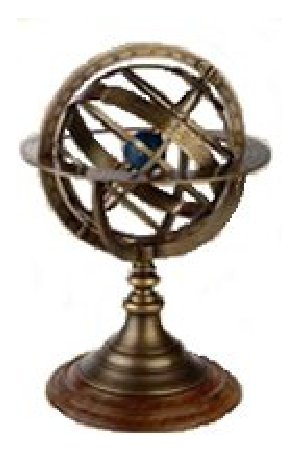
\includegraphics[height=3cm]{sphere} & 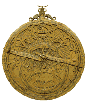
\includegraphics[height=3cm]{astrolabe} & 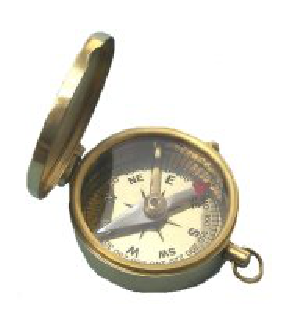
\includegraphics[height=3cm]{boussole}  & 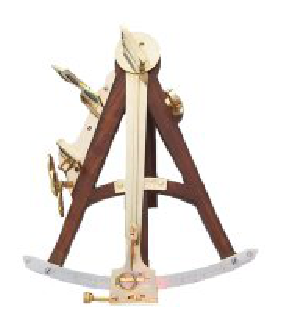
\includegraphics[height=3cm]{octant} & 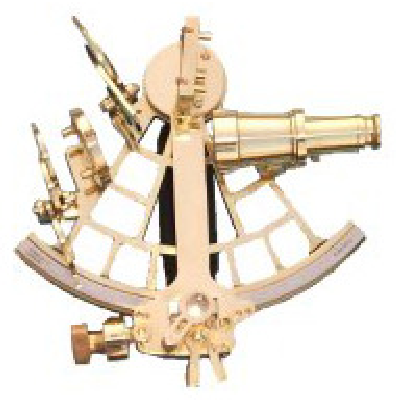
\includegraphics[height=3cm]{sextant} \\
        Sphère armillaire : & Astrolabe : & Boussole : & Octant : & Sextant : \\
        modélisation de la sphère céleste & représentation plane de la sphère armillaire & indique le nord magnétique & mesure la hauteur des corps célestes (\udeg{45}) & mesure la hauteur des corps célestes (\udeg{60}) \\
        & & & & \\
        Antiquité & Antiquité & {\small XIII}\up{e} & {\small XVIII}\up{e} & {\small XVIII}\up{e} \\
     \end{tabular}}
   \end{center}
   \bigskip
   \begin{cadre}[B2][J4]
      \begin{center}
         Vidéo : \href{https://www.yout-ube.com/watch?v=E0KvuFx0Mr8}{\bf Du kamal au GPS 1} et \href{https://www.youtube.com/watch?v=Jv21tvyZokk}{\bf Du kamal au GPS 2}, chaîne Youtube du {\it Musée national de la marine}. 
      \end{center}
   \end{cadre}
\end{debat}


%%%%%%%%%%%%%%%%%%%%%%%
%%%%%%%%%%%%%%%%%%%%%%%
\activites

\begin{activite}[Avec des allumettes]
   {\bf Objectifs :} construire des triangles sous contraintes.
   \begin{QCM}
      Devant vous, vous avez dix allumettes. Pour chacune des questions suivantes, faire la construction si elle est possible avec des allumettes puis faire un dessin pour schématiser la situation.
      \begin{enumerate}
         \item
         \begin{enumerate}
            \item Aligner quatre allumettes en les plaçant les unes à côté des autres.
            \bigskip
            \begin{center}
               
\includegraphics[width=3cm]{allumette}
\includegraphics[width=3cm]{allumette}
\includegraphics[width=3cm]{allumette}
\includegraphics[width=3cm]{allumette}
            \end{center}
            \bigskip
            \item À partir de ce segment de longueur 4 allumettes, construire un triangle dont les deux autres côtés ont pour longueur trois allumettes. \\ [2cm]
            \item En utilisant les dix allumettes, construire un triangle différent du précédent dont un des côtés a pour longueur quatre allumettes. Quelles sont les longueurs de ses côtés ? \\ [2cm]
         \end{enumerate}
         \item En utilisant les dix allumettes, est-il possible de construire un triangle dont un des côtés a pour longueur six allumettes ? sept allumettes ? Expliquer. \\ [2cm]
         \item En utilisant les dix allumettes, peut-on construire un triangle dont un côté a pour longueur cinq allumettes ? Que constate-t-on dans ce cas ? \\ [2cm]
         \item On veut maintenant construire un triangle de périmètre 15 allumettes dont les côtés ont pour longueur un nombre entier d'allumettes. Donner toutes les solutions possibles. \\ [2cm]
      \end{enumerate}
   \end{QCM}
\end{activite}


%%%%%%%%%%%%%%%%%%%%%%%%%%%%%%
%%%%%%%%%%%%%%%%%%%%%%%%%%%%%%
\cours 

%%%%%%%%%%%%%%%%
\section{L'inégalité triangulaire}

\begin{propriete}
   Dans un triangle, la longueur d'un côté est toujours inférieure à la somme des longueurs des deux autres côtés. S'il y a égalité, alors les trois points sont alignés et le triangle est \og plat \fg.
\end{propriete}

\medskip

\begin{exemple}
   \begin{center}
   {\small
      \begin{pspicture}(0,-0.3)(3.5,2)
         \pstGeonode[CurveType=polygon,PointSymbol=none,PosAngle={180,90,0}](0,0){A}(2.5,2){C}(3.5,0){B}
         \pstLabelAB[offset=-3mm]{A}{B}{\ucm{3,5}}
         \pstLabelAB{A}{C}{\ucm{3,2}}
         \pstLabelAB{C}{B}{\ucm{2,2}}
      \end{pspicture}}
   \end{center}
   \correction
   Dans le triangle $ABC$, on a :
   \begin{itemize}
      \item $AC =\ucm{3,2}$ et $AB+BC =\ucm{5,7}$ donc $AC\leq AB+BC$ ;
      \item $CB =\ucm{2,2}$ et $CA+AB =\ucm{6,7}$ donc $CB\leq CA+AB$ ;
      \item $BA =\ucm{3,5}$ et $BC+CA =\ucm{5,4}$ donc $BA\leq BC+CA$.
   \end{itemize}
\end{exemple}

\smallskip

\begin{remarque}
   dans la pratique, on vérifie seulement que la longueur du plus grand côté est plus grande que la somme des longueurs des deux autres côtés.
\end{remarque}


%%%%%%%%%%%%%%%%%
\section{Construction de triangles}

Pour construire un triangle, il faut au minimum trois données : \\
   - soit trois longueurs ; \\
   - soit deux longueurs et l'angle compris entre les segments correspondants aux longueurs données ; \\
   - soit une longueur et les deux angles adjacents au segment correspondant à la longueur donnée ; \\
   - si on a trois angles, on pourra construire un triangle mais il ne sera pas unique : tous les triangles seront semblables (des agrandissements ou des réductions du même triangle).

\bigskip

\begin{methode*1}[Construction d'un triangle connaissant trois longueurs]
   Pour construire un triangle $ABC$ dont on connaît les longueurs des trois côtés :
   \begin{itemize}
      \item on trace à la règle graduée l'un des côtés (en général le plus grand), par exemple $[AB]$ ;
      \item on trace un arc de cercle de centre $A$ et de rayon $AC$ ;
      \item on trace un arc de cercle de centre $B$ et de rayon $BC$ ;
      \item le point $C$ se situe à l'intersection des deux arcs de cercle.
   \end{itemize}
   \exercice
      Tracer le triangle $ABC$ tel que : $AB =\ucm{3,5}$ ; $BC =\ucm{2,2}$ ; $CA =\ucm{3,2}$.
   \correction
         \ \\
         {\small
         \psset{unit=0.8}
         \begin{pspicture}(-0.5,-1.5)(4.8,2.8)
            \pstGeonode[PosAngle={225,-45}](0,0){A}(3.5,0){B}
            \pstLineAB{A}{B}
            \pstLabelAB[offset=-3mm]{A}{B}{\ucm{3,5}}
         \end{pspicture}
         \begin{pspicture}(0,-1.5)(4.8,2.8)
            \pstGeonode[PosAngle={225,-45}](0,0){A}(3.5,0){B}
            \pstLineAB{A}{B}
            \psset{linecolor=A1}
            \psarc(0,0){3.2}{30}{60}
            \rput{55}(0.8,1.3){\textcolor{A1}{\ucm{3,2}}}
            \compas{1.5}{1.2}{55}{0.9}{34.5}
         \end{pspicture}
         \begin{pspicture}(0,-1.5)(4.8,2.8)
            \pstGeonode[PosAngle={225,-45}](0,0){A}(3.5,0){B}
            \pstLineAB{A}{B}
            \psset{linecolor=A1}
            \psarc(0,0){3.2}{30}{60}
            \psset{linecolor=B1}
            \psarc[fillstyle=none](3.5,0){2.2}{90}{130}
            \rput{-45}(2.8,0.8){\textcolor{B1}{\ucm{2,2}}}
            \compas{3.3}{1.1}{130}{0.9}{23}
         \end{pspicture}
         \begin{pspicture}(0,-1.5)(2,2.8)
            \pstGeonode[CurveType=polygon,PointSymbol=none,PosAngle={225,90,-45}](0,0){A}(2.5,2){C}(3.5,0){B}
         \end{pspicture}}
\end{methode*1}

\begin{methode*1}[Construction d'un triangle connaissant deux longueurs et un angle]
   Pour construire un triangle $ABC$ dont on connait la longueur de deux côtés ainsi que l'angle entre ces cotés :
   \begin{itemize}
      \item on trace à la règle graduée l'un des côtés donnés, par exemple $[AB]$ ;
      \item on trace au rapporteur l'angle donné à partir du segment tracé ;
      \item on trace à la règle graduée le deuxième segment de longueur donnée le long du support de l'angle tracé juste avant ;
      \item le point $C$ se trouve à l'extrémité de ce segment.
   \end{itemize}
   \exercice
      Tracer le triangle $ABC$ tel que : $AB =\ucm{3,5}$ ; $\widehat{BAC} =39$\degre et $CA =\ucm{3,2}$.
   \correction
     \ \\
      {\small
      \psset{unit=0.8}
      \begin{pspicture}(-0.5,-1.5)(4.5,3)
         \pstGeonode[PosAngle={225,-45}](0,0){A}(3.5,0){B}
         \pstLineAB{A}{B}
         \pstLabelAB[offset=-3mm]{A}{B}{\ucm{3,5}}
      \end{pspicture}
      \begin{pspicture}(-3,-1.5)(4.1,3)
         \pstGeonode[PosAngle={225,-45}](0,0){A}(3.5,0){B}
         \pstLineAB{A}{B}  
         \psset{linecolor=A1}
         \rapporteur{0}{0}{0}{0.75}
         \psline(0,0)(4;38.66)
         \psarc(0,0){1}{0}{39}
         \rput(1.4,0.4){\textcolor{A1}{39\degre}}
      \end{pspicture}
      \begin{pspicture}(-1,-1.5)(3,3)
         \pstGeonode[CurveType=polygon,PointSymbol=none,PosAngle={225,90,-45}](0,0){A}(2.5,2){C}(3.5,0){B}
         \psline(0,0)(4;38.66) 
         \psline[linecolor=B1,linewidth=0.8mm](0,0)(2.5,2)
         \rput{40}(1.1,1.4){\textcolor{B1}{3,2 cm}}
      \end{pspicture}}
\end{methode*1}

\ \\ [5mm]

\begin{methode*1}[Construction d'un triangle connaissant une longueur et deux angles]
   Pour construire un triangle $ABC$ dont on connait la longueur d'un côté ainsi que ses deux angles adjacents :
   \begin{itemize}
      \item on trace à la règle graduée le côté donné, par exemple $[AB]$ ;
      \item on trace au rapporteur les deux angles donnés à partir du segment tracé ;
      \item les deux demi-droites tracées grâce au rapporteur se coupent au point $C$.
   \end{itemize}
   \exercice
      Tracer le triangle $ABC$ tel que : $AB =\ucm{3,5}, \widehat{BAC} =39$\degre et $\widehat{ABC} =63$\degre
   \correction
      \ \\
      {\small
      \psset{unit=0.8}
      \begin{pspicture}(-0.5,-1.5)(4.5,3.3)
         \pstGeonode[PosAngle={225,-45}](0,0){A}(3.5,0){B}
         \pstLineAB{A}{B}
         \rput(1.75,-0.25){3,5 cm}
      \end{pspicture}
      \begin{pspicture}(-3,-1.5)(4.1,3.3)
         \pstGeonode[PosAngle={225,-45}](0,0){A}(3.5,0){B}
         \pstLineAB{A}{B}  
         \psset{linecolor=A1}
         \rapporteur{0}{0}{0}{0.75}
         \psline(0,0)(4;38.66)
         \psarc(0,0){1}{0}{39}
         \rput(1.4,0.4){\textcolor{A1}{39\degre}}
      \end{pspicture}
      \begin{pspicture}(-1,-1.5)(3,3.3)
         \pstGeonode[PointSymbol=none,PosAngle={225,-45}](0,0){A}(3.5,0){B}
         \pstLineAB{A}{B}
         \psline{->}(2.5,3.2)(2.5,2)
         \psset{linecolor=A1}
         \psline(0,0)(4;38.66)
         \psset{linecolor=B1}
         \rapporteur{4.65}{0}{0}{0.75}
         \psline(3.5,0)(2.05,2.8)
         \psarc(3.5,0){0.8}{117}{180}
         \rput(2.5,0.6){\textcolor{B1}{63\degre}}
         \rput(2.5,3.5){C}
      \end{pspicture}}
\end{methode*1}

\ \\

\begin{remarque}
   pour chaque cas, on a deux choix de construction pour $C$, d'un côté ou de l'autre du segment.
\end{remarque}


%%%%%%%%%%%%%%%%%%%%%%%%%
%%%%%%%%%%%%%%%%%%%%%%%%%
\exercicesbase

\begin{colonne*exercice}

\begin{exercice} %1
   Ces triangles sont-ils constructibles (ils ne sont pas tracés en vraie grandeur) ?
   \begin{center}
      {\small
      \begin{pspicture}(-0.5,-0.5)(3,2.5)
         \pstTriangle[PointSymbol=none](0,0){G}(3,0){L}(1,2){E}
         \pstLabelAB[offset=-3mm]{G}{L}{\ucm{8}}
         \pstLabelAB{G}{E}{\ucm{3}}
         \pstLabelAB{E}{L}{\ucm{3,5}}
      \end{pspicture}
      \begin{pspicture}(-0.5,-1.5)(3.5,1)
         \pstTriangle[PointSymbol=none](0,0){E}(3,0){U}(1.5,1){A}
         \pstLabelAB[offset=-3mm]{E}{U}{\ucm{6,2}}
         \pstLabelAB{E}{A}{\ucm{3,1}}
          \pstSegmentMark[MarkAngle=90]{E}{A}
          \pstSegmentMark[MarkAngle=90]{A}{U}
      \end{pspicture} 
   
      \psset{unit=1.5}
      \begin{pspicture}(0,-1)(3,1.5)
         \pstTriangle[PointSymbol=none](0,0){G}(3,0){Z}(2.7,1){A}
         \pstLabelAB[offset=-3mm]{G}{Z}{\ucm{6,3}}
         \pstLabelAB{A}{Z}{\ucm{2}}
         \pstSegmentMark[MarkAngle=90]{Z}{G}
         \pstSegmentMark[MarkAngle=90]{A}{G}
      \end{pspicture} 
      \begin{pspicture}(-0.5,-0.5)(3.5,1.5)
         \pstTriangle[PointSymbol=none](0,0){A}(3,0){R}(1,1.5){I}
         \pstLabelAB[offset=-3mm]{A}{R}{\udm{1,3}}
         \pstLabelAB{A}{I}{\ucm{6}}
         \pstLabelAB{I}{R}{\ucm{8}}
      \end{pspicture}}
   \end{center}
\end{exercice}

\begin{corrige}
   \begin{itemize}
      \item Triangle $GEL$ : le plus grand côté $GL$ mesure \ucm{8} et la somme des deux autres côtés vaut $\ucm{3}+\ucm{3,5} =\ucm{6,5}$ qui est inférieure à \ucm{8} donc, {\blue le triangle $GEL$ n'est pas constructible}. \smallskip
      \item Triangle $EAU$ : le plus grand côté $EU$ mesure \ucm{6,2} et la somme des deux autres côtés vaut $\ucm{3,1}+\ucm{3,1} =\ucm{6,2}$ qui est égale à \ucm{6,2} donc, {\blue le triangle $EAU$ est constructible, mais il est plat}. \smallskip
      \item Triangle $GAZ$ : le plus grand côté $GZ$ mesure \ucm{6,3} et la somme des deux autres côtés vaut $\ucm{6,3}+\ucm{2} =\ucm{8,3}$ qui est supérieure à \ucm{6,3} donc, {\blue le triangle $GAZ$ est constructible}. \smallskip
      \item Triangle $AIR$ : le plus grand côté $AR$ mesure \ucm{13} et la somme des deux autres côtés vaut $\ucm{6}+\ucm{8} =\ucm{14}$ qui est supérieure à \ucm{13} donc, {\blue le triangle $AIR$ est constructible}.
   \end{itemize}
\end{corrige}

\bigskip


\begin{exercice} %2
   Choisir trois nombres du tableau (chacun une fois) correspondant aux longueurs des côtés d'un triangle :
   \begin{enumerate}
      \item non constructible ;
      \item quelconque ;
      \item isocèle ;
      \item de périmètre \ucm{13}.
   \end{enumerate}
   \begin{center}
   {\hautab{2}
   \begin{tabular}{|*{4}{C{1}|}}
      \hline
      \ucm{8} & \ucm{5} & \ucm{12} & \ucm{2} \\
      \hline
      \ucm{10} & \ucm{12} & \ucm{15} & \ucm{10} \\
      \hline
      \ucm{9} & \ucm{3} & \ucm{5} & \ucm{7} \\
      \hline
   \end{tabular}}
   \end{center}
\end{exercice}

\begin{corrige}
   On a, par exemple (solution non unique) un triangle :
   \begin{enumerate}
      \item non constructible : {\blue \ucm{15} ; \ucm{8} et \ucm{2}}.
      \item quelconque : {\blue \ucm{10} ; \ucm{9} et \ucm{7}}.
      \item isocèle : {\blue \ucm{12} ; \ucm{12} et \ucm{10}}.
      \item de périmètre \ucm{13} : {\blue \ucm{5} ; \ucm{5} et \ucm{3}}.
   \end{enumerate}
\end{corrige}

\bigskip


\begin{exercice} %3
   Le périmètre d'un triangle non aplati est de \ucm{18}. Ce triangle peut-il avoir un côté\dots
   \begin{colenumerate}{2}
      \item de \ucm{7} ?
      \item de \ucm{4} ?
      \item de \ucm{11} ?
      \item de \ucm{9} ?
   \end{colenumerate}
   Justifier en donnant un exemple lorsque cela est possible ou en le prouvant dans le cas contraire.
\end{exercice}

\begin{corrige}
   \ \\ [-5mm]
   \begin{enumerate}
      \item Avec un côté de \ucm{7}, il reste \ucm{11}. On peut choisir les deux autres côtés de mesures \ucm{6} et \ucm{5} par exemple. {\blue Ce triangle est  constructible} puisque $\ucm{6}+\ucm{5} =\ucm{11} >\ucm{7}$. \smallskip
      \item Avec un côté de \ucm{4}, il reste \ucm{14}. On peut choisir les deux autres côtés de mesures \ucm{7} et \ucm{7} par exemple. {\blue Ce triangle est constructible} puisque $\ucm{7}+\ucm{4} =\ucm{11} >\ucm{7}$. \smallskip
      \item Avec un côté de \ucm{11}, il reste \ucm{7}. On ne peut pas construire un triangle car \ucm{7} est inférieur à \ucm{11}. {\blue Ce triangle n'est pas constructible}. \smallskip
      \item Avec un côté de \ucm{9}, il reste \ucm{9}. On peut choisir les deux autres côtés de mesures \ucm{4} et \ucm{5} par exemple. {\blue Ce triangle est un triangle plat} puisque $\ucm{4}+\ucm{5} =\ucm{9}$.
   \end{enumerate}
\end{corrige}

\bigskip


\begin{exercice} %4
   Construire en vraie grandeur les deux triangles $NOM$ et $EDF$ suivants tels que :
   \begin{enumerate}
      \item $MN =\ucm{4,5}$, $MO =\ucm{7}$ et $\widehat{NMO} =\udeg{48}$.
      \item $\widehat{FDE} =\udeg{45}$, $DE =\ucm{8}$ et $\widehat{FED} =\udeg{28}$.
   \end{enumerate}
\end{exercice}

\begin{corrige}
   \ \\ [-5mm]
   \begin{enumerate}
      \psset{linecolor=blue}
      \item Triangle $NOM$ : \\
         \begin{pspicture}(0,-1)(7,4)
            \pstTriangle[PointSymbol=none](0,0){M}(7,0){O}(4.5;48){N}
            \pstLabelAB[offset=-3mm]{M}{O}{\small\blue \ucm{7}}
            \pstLabelAB{M}{N}{\small\blue \ucm{4,5}}
            \pstMarkAngle{O}{M}{N}{\small\blue \udeg{48}}
         \end{pspicture}
      \item Triangle $EDF$ : \\
         \begin{pspicture}(0.25,-0.5)(8,3.5)
            \pstTriangle[PointSymbol=none](0,0){D}(8,0){E}(3.93;45){F}
            \pstLabelAB[offset=-3mm]{D}{E}{\small\blue \ucm{8}}
            \pstMarkAngle{E}{D}{F}{\small\blue \udeg{45}}
            \pstMarkAngle{F}{E}{D}{\small\blue \udeg{28}}
         \end{pspicture}
   \end{enumerate}
\end{corrige}

\bigskip


\begin{exercice} %5
   Après avoir effectué les calculs nécessaires, tracer chacun des triangles suivants en vraie grandeur.
   \begin{enumerate}
      \item $EFG$ tel que $EF =\ucm{7,5}$, $\widehat{EFG}=\udeg{49}$ et $\widehat{EGF}=\udeg{72}$.
      \item $RST$ isocèle en $S$ de périmètre \ucm{13} et $ST=\ucm{4}$.
      \item $OCI$ isocèle en $I$ tel que $CO=\ucm{7}$ et $\widehat{CIO} =\udeg{100}$.
   \end{enumerate}
\end{exercice}

\begin{corrige}
   \ \\[-5mm]
   \begin{enumerate}
   \psset{linecolor=blue}
      \item Pour tracer le triangle $EFG$, il faut calculer l'angle $\widehat{GEF}$ : la somme des angle d'une triangle faisant \udeg{180}, $\widehat{GEF} =\udeg{180}-\udeg{49}-\udeg{72} =\udeg{59}$. \\
         \begin{pspicture}(0.25,-0.75)(7.5,6)
            \pstTriangle[PointSymbol=none](0,0){E}(7.5,0){F}(5.95;59){G}
            \pstLabelAB[offset=-3mm]{E}{F}{\small\blue \ucm{7,5}}
            \pstMarkAngle{G}{F}{E}{\small\blue \udeg{49}}
            \pstMarkAngle{E}{G}{F}{\small\blue \udeg{72}}
            \pstMarkAngle{F}{E}{G}{\small \udeg{59}}
         \end{pspicture}
      \item Pour tracer le triangle $RST$ isocèle en $S$, il faut calculer la mesure du troisième côté. \\
      On a $SR =ST =\ucm{4}$ et le périmètre mesure \ucm{13} donc, $RT =\ucm{13}-2\times\ucm{4} =\ucm{5}$. \\
   \end{enumerate}
   
\Coupe

         \begin{pspicture}(-1,-0.75)(5,3.75)
            \pstTriangle[PointSymbol=none](0,0){T}(5,0){R}(2.5,3.12){S}
            \pstLabelAB[offset=-3mm]{T}{R}{\small \ucm{5}}
            \pstLabelAB{T}{S}{\small\blue \ucm{4}}
            \pstLabelAB{S}{R}{\small \ucm{4}}
         \end{pspicture}  
   \begin{enumerate}
   \setcounter{enumi}{2}      
      \item Pour tracer le triangle $OCI$, il faut calculer les angles à la base. La somme des angle faisant \udeg{180}, il reste $\udeg{180}-\udeg{100} =\udeg{80}$ à partager en deux angles égaux puisque le triangle est isocèle, soit \udeg{40} chacun. \\
         \begin{pspicture}(0,0)(7,3.5)
            \pstTriangle[PointSymbol=none](0,0){C}(7,0){O}(4.57;40){I}
            \pstLabelAB[offset=-3mm]{C}{O}{\small\blue \ucm{7}}
            \pstMarkAngle{C}{I}{O}{\small\blue \udeg{100}}
            \pstMarkAngle{O}{C}{I}{\small \udeg{40}}
            \pstMarkAngle{I}{O}{C}{\small \udeg{40}}
         \end{pspicture}
   \end{enumerate}
\end{corrige}

\bigskip


\begin{exercice} %6
   Loutfi a trouvé un triangle sympa dont tous les angles ont pour mesure un entier pair : \udeg{44}, \udeg{66} et \udeg{70}.
   \begin{enumerate}
      \item Trouver un autre exemple de triangle dont les mesures d'angles sont paires.
      \item En poursuivant ses recherches, elle a trouvé un triangle dont les mesures sont des multiples de trois : 45\degre, 51\degre et 84\degre. Trouve un autre exemple de triangle dont les mesures d'angles sont des multiples de trois.
      \item Continuer les recherches en trouvant un triangle dont les mesures d'angles sont des multiples de quatre.
      \item Cela est-il possible avec tous les nombres entiers ?
   \end{enumerate}
\end{exercice}

\begin{corrige}
   \ \\ [-5mm]
   \begin{enumerate}
      \item On peut choisir, par exemple, {\blue $\udeg{60} ; \udeg{60}$ et $\udeg{60}$}.
      \item On peut choisir, par exemple, {\blue $\udeg{30} ; \udeg{60}$ et $\udeg{90}$}.
      \item On peut choisir, par exemple, {\blue $\udeg{40} ; \udeg{60}$ et $\udeg{80}$}.
      \item {\blue Non}, cela n'est pas possible par exemple avec des multiples de 7 : dans ce cas, la somme des angles est un multiple de 7 et doit être égale à \udeg{180} ce qui n'est pas possible puisque 7 n'est pas un diviseur de 180.
   \end{enumerate}
\end{corrige}

\bigskip


\begin{exercice} %7
   Meriem veut tracer un triangle tel que son périmètre mesure \ucm{16} et deux de ses angles mesurent \udeg{64} et \udeg{46}.
   \begin{enumerate}
      \item Calculer la mesure de son troisième angle.
      \item Tracer un segment $[DE]$ mesurant \ucm{16} et placer le point $A$ tel que $\widehat{ADE} =\udeg{32}$ et $\widehat{AED} =\udeg{23}$ qui sont les angles moitié de \udeg{64} et \udeg{46}.
      \item Placer un point $B$ sur le segment $[DE]$ à égale distance de $A$ et de $D$, puis un point $C$ sur le segment $[DE]$ à égale distance de $A$ et $E$. 
      \item Quelle est la nature des triangles $ABD$ et $ACE$ ?
      \item Calculer la mesure des angles de $ABD$ et de $ACE$.
      \item Démontrer que le périmètre du triangle $ABC$ vaut bien \ucm{16}.
      \item Montrer que $\widehat{ABC} =\udeg{46}$ et $\widehat{ACB} =\udeg{64}$ puis conclure.
   \end{enumerate}
\end{exercice}

\begin{corrige}
   \ \\ [-5mm]
    \begin{enumerate}
      \item La somme des angles fait \udeg{180} donc, le troisième angle mesure $\udeg{180}-\udeg{64}-\udeg{46} =\blue\udeg{70}$.
      \item Figure à l'échelle 1/2 en bas de page, complétée au fur et à mesure.
      \item Pour tracer les points demandés, il suffit de construire la médiatrice de $[AD]$ qui coupe $[DE]$ en $B$, puis celle de $[AE]$ qui coupe $[DE]$ en $C$.
      \item {\blue Le triangle $ABD$ est isocèle en $B$} puisque le point $B$ est à égale distance de $A$ et $D$. \\
         {\blue Le triangle $ACE$ est isocèle en $C$} puisque le point $C$ est à égale distance de $A$ et $E$.
   \end{enumerate}
   
\Coupe

   \begin{enumerate}
   \setcounter{enumi}{4}
      \item $ABD$ est isocèle en $B$ donc, $\widehat{DAB} =\widehat{ADB} =\udeg{32}$. \\
         La somme des angles faisant \udeg{180}, l'angle $\widehat{ABD}$ mesure alors $\udeg{180}-2\times\udeg{32} =\udeg{116}$. \\
         {\blue Les angles de $ABD$ mesurent \udeg{32}, \udeg{32} et \udeg{116}}. \\
         $ACE$ est isocèle en $C$ donc, $\widehat{CAE} =\widehat{CEA} =\udeg{23}$. \\
         La somme des angles faisant \udeg{180}, l'angle $\widehat{ACE}$ mesure $\udeg{180}-2\times\udeg{23} =\udeg{134}$. \\
         {\blue Les angles de $ACE$ mesurent \udeg{23}, \udeg{23} et \udeg{134}}.
      \item $AB+BC+CA = DB+BC+CE =DE =\ucm{16}$. \\
        {\blue Le périmètre de $ABC$ vaut \ucm{16}}.
      \item $\widehat{ABC} =\udeg{180}-\udeg{116} =\udeg{64}$ ; \\
         $\widehat{ACB} =\udeg{180}-\udeg{134} =\udeg{46}$. \\
         Conclusion : {\blue le triangle $ABC$ correspond bien au triangle demandé.}
   \end{enumerate}
   {\psset{unit=0.5,PointSymbol=none,CodeFig=true}
      \small
       \begin{pspicture}(1,-2.3)(15.5,5.5)
         \pstTriangle[PointSymbol=none](0,0){D}(16,0){E}(7.63;32){A}
         \psline[linestyle=dashed]{<->}(0,-1.5)(16,-1.5)
         \rput(8,-2){\ucm{16}}
         \pstMarkAngle[MarkAngleRadius=1.5,LabelSep=2.2]{E}{D}{A}{\small \udeg{32}}
         \pstMarkAngle[MarkAngleRadius=1.5,LabelSep=2.2]{A}{E}{D}{\small \udeg{23}}
         \psset{CodeFigColor=B1,linecolor=B1}
         \pstMediatorAB[PointName=none]{A}{D}{I}{J}
         \pstMediatorAB[PointName=none,SegmentSymbol=pstslash]{E}{A}{K}{L}
         \psset{PosAngle=-90,linecolor=blue}
         \pstInterLL{D}{E}{I}{J}{B}
         \pstInterLL{D}{E}{K}{L}{C}
         \pstLineAB{A}{B}
         \pstLineAB{A}{C}
         \pstLineAB{B}{C}
         \pstMarkAngle[MarkAngleRadius=0.8,LabelSep=1.6]{C}{B}{A}{\small\blue \udeg{64}}
         \pstMarkAngle[MarkAngleRadius=0.8,LabelSep=1.6]{A}{C}{B}{\small\blue \udeg{46}}
      \end{pspicture}}
\end{corrige}

\hfill {\it\footnotesize Source : Sesamath, le manuel 5\up{e}. Génération 5 - 2013}   
\end{colonne*exercice}


%%%%%%%%%%%%%%%%%%%%%%%%%%%%
%%%%%%%%%%%%%%%%%%%%%%%%%%%%
\Recreation

\begin{enigme}[Le tangram]

\partie[histoire]
   Le jeu de tangram, appelé en chinois \og qī qiǎo bǎn \fg, prononcé {\it tzi tchiao pan}, \og les sept plaques de l’habileté \fg, semble avoir été inventé au début du {\small XIX}\up{e} siècle en Chine. \\
   Ce jeu viendrait d'une légende qui dit qu'un empereur chinois du {\small XVI}\up{e} siècle du nom de {\it Tan}, fit tomber un carreau de faïence qui se brisa en 7 morceaux. Il n'arriva jamais à rassembler les morceaux pour reconstituer le carreau mais l'homme s'aperçut qu'avec les 7 pièces il était possible de créer de formes multiples.
   
\vfill

\partie[le tangram carré]
   \begin{minipage}{10cm}
      Voilà le tangram. \\
      Donner la mesure de tous les angles présents sur la figure. \\
      {\it Matériel autorisé : équerre et compas.}
   \end{minipage}
   \qquad
   \begin{minipage}{6cm}
      \psset{unit=0.4}
      \begin{pspicture}(-3,6)(12,10.5)
         \rput{135}(12,0){\gt}
         \rput{-135}(12,12){\gt}
         \rput{-90}(0,0){\pa}
         \rput{45}(3,3){\pt}
         \rput{45}(6,6){\ca}
         \rput{-45}(6,12){\pt}
         \rput{180}(6,12){\mt}
      \end{pspicture}
   \end{minipage}
   
 \vfill
 
\partie[puzzles]
   Le bonhomme et le sapin sont deux formes constituées des sept \\
   pièces du tangram. Tracer le contour des formes à l'intérieur. \\
   {\it Matériel autorisé : règle non graduée et rapporteur.}
\begin{center}
   \psset{unit=0.5}
   \begin{pspicture}(-2,1)(14,25)
      \pspolygon(1.76,0)(6,0)(6,4.24)(9,1.24)(12,4.24)(6,4.24)(6,7.75)(14.49,16.24)(8.12,16.24)(8.12,20.48)(10.24,20.48)(6,24.72)(1.76,20.48)(3.88,20.48)(3.88,16.24)(0,16.24)(-3,13.24)(3,13.24)(0,10.24)(6,4.24)
   \end{pspicture}
\quad
   \begin{pspicture}(-8,-1)(7,23)
      \pspolygon(-2.12,0)(2.12,0)(2.12,4.24)(8.48,4.24)(4.24,8.48)(8.48,8.48)(0,17)(-8.48,8.48)(-4.24,8.48)(-8.48,4.24)(-2.12,4.24)
   \end{pspicture}
\end{center}
\end{enigme}

\begin{corrige}
{\psset{unit=0.4}
   \footnotesize
   \begin{pspicture}(-3,-1)(12,12.3)
      \rput{135}(12,0){\gt}
      \rput{-135}(12,12){\gt}
      \rput{-90}(0,0){\pa}
      \rput{45}(3,3){\pt}
      \rput{45}(6,6){\ca}
      \rput{-45}(6,12){\pt}
      \rput{180}(6,12){\mt}
      \rput(1.5,0.5){\blue\udeg{45}}
      \rput(10.5,0.5){\blue\udeg{45}}
      \rput(6,5){\blue\udeg{90}}
      \rput(11.4,1.7){\blue\udeg{45}}
      \rput(11.4,10.5){\blue\udeg{45}}
      \rput(10.8,11.5){\blue\udeg{45}}
       \rput(9.2,10){\blue\udeg{90}}
      \rput(7.5,11.5){\blue\udeg{45}}
      \rput(4.7,11.5){\blue\udeg{45}}
      \rput(0.8,11.5){\blue\udeg{90}}
      \rput(0.7,7.4){\blue\udeg{45}}
      \rput(0.8,5.8){\blue\udeg{135}}
      \rput(0.7,1.4){\blue\udeg{45}}
      \rput(2.4,7.6){\blue\udeg{45}}
      \rput(2.2,3){\blue\udeg{135}}
      \rput(3.65,4.3){\blue\udeg{45}}
      \rput(3.65,7.5){\blue\udeg{45}}
      \rput(5.1,6){\blue\udeg{90}}
      \rput(6.15,6.8){\blue\udeg{90}}
      \rput(6,11.1){\blue\udeg{90}}
      \rput(4,9){\blue\udeg{90}}
      \rput(8,9){\blue\udeg{90}}
      \rput(7.1,6){\blue\udeg{90}}
   \end{pspicture}}
   
   {\psset{unit=0.2}
   \begin{pspicture}(-3,1)(15,25)
      \rput{-135}(6,16.24){\gt}
      \rput{180}(14.49,16.24){\gt}
      \rput{135}(10.24,20.48){\mt}
      \rput{0}(1.76,0){\pt}
      \rput{-45}(6,4.24){\pt}
      \rput{0}(3.88,16.24){\ca}
      \rput{0}(6,16.24){\pas}
   \end{pspicture}
   \begin{pspicture}(-8,-2)(8,20)
      \rput{0}(-8.49,4.24){\gt}
      \rput{-90}(0,12.73){\gt}
      \rput{45}(0,12.73){\pa}
      \rput{90}(4.24,8.48){\pt}
      \rput{0}(-2.12,0){\ca}
      \rput{-90}(4.24,12.73){\pt}
      \rput{135}(4.24,12.73){\mt}
   \end{pspicture}}
\end{corrige}

